\documentclass{article}

\usepackage[english]{babel}

\usepackage[letterpaper,top=2cm,bottom=2cm,left=3cm,right=3cm,marginparwidth=1.75cm]{geometry}

\usepackage{graphicx}
\usepackage[colorlinks=true, allcolors=blue]{hyperref}

\title{Modul 2 - Static Website}
\author{}

\begin{document}
\begin{figure}[h]
\centering

\includegraphics[width=0.3\textwidth]{logo.png}
\end{figure}
\centering
{\huge
Lomba Kompetensi Siswa\\
Sekolah Menengah Kejuruan\\
Tingkat Provinsi Jawa Barat\\
Tahun 2022\\
\vspace{10mm} %5mm vertical space
}
\vspace{30mm} %5mm vertical space
{\let\newpage\relax\maketitle}
\vspace{30mm} %5mm vertical space
{\LARGE Bidang Lomba Cloud Computing}

\thispagestyle{empty}
\newpage
\raggedright
\pagenumbering{arabic}

\section{Overview}
You have been tasked to deploy a front-end web application on AWS. The application is built using Next.js without server-side rendering, thus can be be hosted on S3. The application also requires API call to previous task (modul 1). If you fail to deploy the previous task, please ask us for a working API endpoint.

\section{General Rules}
\begin{enumerate}
    \item Failure to comply with the rules will result in immediate disqualification.
    \item You have 2 hours to finish the tasks.
    \item You may not open any website unless otherwise specified in section \ref{references} and you may open the control panel of your domain provider to update the nameserver to Route 53.
    \item You may use AWS Console and AWS CLI to deploy the solutions. You may not use SAM, CloudFormation or CDK.
    \item Between and after the event, you may not access your account. Any activity on your AWS account during this period is not allowed.
    \item During the event, multiple login is not permitted.
    \item This module requires compilation, you can use an EC2 instance or your own computer to compile the project.
    \item If you have any question, do not hesitate to ask.
\end{enumerate}
\section{Architecture}
\begin{figure}[h]
\centering
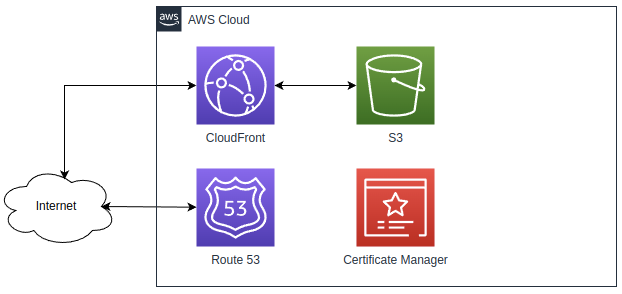
\includegraphics[width=\textwidth]{modul2_architecture.png}
\caption{\label{fig:architecture}Architecture Diagram}
\end{figure}

\section{Information}\label{information}
\begin{enumerate}
    \item The repository URL for the project is \href{https://github.com/kensasongko/lksccjabar2022modul2_aplikasi}{https://github.com/kensasongko/lksccjabar2022modul2\_aplikasi}
    \item The URL for the CloudFront Function code is \href{https://gist.github.com/kensasongko/610912a2b9a645b00743c773a00848ea}{https://gist.github.com/kensasongko/610912a2b9a645b00743c773a00848ea}
    \item This solution must be deployed in \textbf{us-east-1 (N. Virginia) region}. Deploying in another region will result in a major point reduction.
\end{enumerate}
\section{Task}
\begin{enumerate}
    \item Create a standard S3 bucket with the following specifications:
    \begin{itemize}
        \item Bucket name: modul2.[YOUR\_DOMAIN]\\
        If the bucket name is taken, you may append a 6-character random string to the end of the bucket name.
        \item Tags: Key=LKS-ID, Value=MODUL2
        \item Block all public access: True
        \item Bucket versioning: Disabled
        \item Server-side encryption: Enabled
        \item Encryption key type: Amazon S3-managed keys
    \end{itemize}
    \item Clone the repository, follow the instruction from README.md to generate the static files. 
    \item Upload the generated static files to the S3 bucket.
    \item Create a CloudFront Distribution with the following specifications:
    \begin{itemize}
        \item Origin domain: Your S3 bucket
        \item Use origin access identity to access the s3 bucket
        \item Enable Origin Shield: No
        \item Viewer protocol policy: Redirect HTTP to HTTPS
        \item Caching Policy: CachingOptimized
        \item Tags: Key=LKS-ID, Value=MODUL2
    \end{itemize}
    \item Create a certificate from ACM using DNS validated
    \begin{itemize}
        \item Domain Name: modul2.[YOUR\_DOMAIN]
        \item Validation Method: DNS validation
        \item Tags: Key=LKS-ID, Value=MODUL2
    \end{itemize}
    \item Configure CloudFront distribution to use custom domain modul2.[YOUR\_DOMAIN].
    \item Create and publish a CloudFront Function using the code provided in number 2 from Section \ref{information}. Associate the function with your distribution.\\
    Make sure you don't have to append index.html to access the website.
    \item Open pages/index.js with any text editor, replace the text "My Simple TODO Application" with "Peserta\_[YOUR\_PARTICIPATION\_ID] Simple TODO Application"
    \item Rebuild and re-export the application, re-upload the static page to the S3 bucket.
    \item Invalidate CloudFront cache to make sure the cache is renewed.
\end{enumerate}

\section{References}\label{references}

\begin{itemize}
    \item \href{https://docs.aws.amazon.com/AmazonS3/latest/userguide/Welcome.html}{S3 documentation}
    \item \href{https://docs.aws.amazon.com/AmazonCloudFront/latest/DeveloperGuide/Introduction.html}{CloudFront documentation}
    \item \href{https://docs.aws.amazon.com/AmazonCloudFront/latest/DeveloperGuide/cloudfront-functions.html}{CloudFront Function documentation}
    \item \href{https://docs.aws.amazon.com/Route53/latest/DeveloperGuide/Welcome.html}{Route 53 documentation}
    \item \href{https://docs.aws.amazon.com/acm/latest/userguide/acm-overview.html}{Certificate Manager documentation}
    \item \href{https://docs.npmjs.com/cli/v8/commands}{npm documentation}
    \item \href{https://classic.yarnpkg.com/en/docs}{yarn documentation}
    \item \href{https://nextjs.org/docs/deployment}{Next.js documentation}
\end{itemize}

\section*{Good luck!}

\end{document}
